\documentclass{beamer}
\usetheme{Rochester} % My favorite!
\usepackage{amsmath}
%\usetheme{Boadilla} % Pretty neat, soft color.
%\usetheme{default}
%\usetheme{Warsaw}
%\usetheme{Bergen} % This template has nagivation on the left
%\usetheme{Frankfurt} % Similar to the default 
%with an extra region at the top.
%\usecolortheme{seahorse} % Simple and clean template
%\usetheme{Darmstadt} % not so good
% Uncomment the following line if you want %
% page numbers and using Warsaw theme%
% \setbeamertemplate{footline}[page number]
%\setbeamercovered{transparent}
%\setbeamercovered{invisible}
% To remove the navigation symbols from 
% the bottom of slides%
\usepackage[T1]{fontenc}
\setbeamertemplate{navigation symbols}{} 
\setbeamertemplate{itemize items}[default]
\usefonttheme[onlymath]{serif}
%\usepackage{biblatex}
\usepackage{graphicx}
\usepackage{sidecap}
\usepackage{xcolor}
\definecolor{blue}{rgb}{0, 0, 1}
\definecolor{red}{rgb}{1, 0, 0}
\definecolor{purple}{rgb}{0.9, 0.1, 0.9}
\definecolor{green}{rgb}{0.3, 0.6, 0.3}
\bibliography{/usr/local/texlive/texmf-local/bibtex/bib/local/library}
%\usepackage{bm}         % For typesetting bold math (not \mathbold)
%\logo{\includegraphics[height=0.6cm]{yourlogo.eps}}
%
\title[Evolution 2014]{Evolution 2014}
\author{Jeremy Berg and Graham Coop}
\institute[UC Davis]
{
University of California, Davis \\
}
\date{June 20, 2014}
% \today will show current date. 
% Alternatively, you can specify a date.
%
\begin{document}


\begin{frame}
\titlepage
\end{frame}

\begin{frame}
	\frametitle{Background Slide(s)}
		\begin{itemize}
			\item We want to know whether a particular trait is adaptively differentiated among populations
			\pause
			\begin{itemize}
				\item Put them in a common garden and measure them
			\end{itemize}
		\end{itemize}
\end{frame}

\begin{frame}
\frametitle{}
	\begin{columns}
		\begin{column}{0.63\textwidth}
			\only<1-1>{\includegraphics[width = \textwidth]{../Figs/two_trait_histo.pdf}}
			\only<2-2>{\includegraphics[width = \textwidth]{../Figs/two_trait_histo_w_lines.pdf}}
			\only<3-5>{\includegraphics[width = \textwidth]{../Figs/two_trait_histo_w_expect.pdf}}
		\end{column}
		\begin{column}{0.38\textwidth}
			\uncover<2-5>{\begin{block}{}
				$Q_{ST} = \frac{\color{green}{V_B}}{\color{green}{V_B} + \color{purple}{V_W}} = \frac{V_B}{V_T}$ \\~\\
				\uncover<3-5>{$F_{ST} = \mathbb{E}\left[\frac{V_B}{V_B + V_W}\right]$} \\~\\
				\uncover<4-5>{$\mathbb{E}[V_B] = \left(\color{green}{V_B} + \color{purple}{V_W} \right) F_{ST}$} \\~\\
				\uncover<5-5>{$\frac{Q_{ST}}{F_{ST}} = \frac{V_B}{\mathbb{E}[V_B]} \sim \chi^2$}
			\end{block}}
		\end{column}
	\end{columns}
\end{frame}


%\begin{frame}
%\frametitle{Quantifying and Testing for Adaptive Differentiation}
%	\begin{block}{Things That End in $ST$}
%		\pause
%		\begin{itemize}
%			\item $F_{ST}$
%				\begin{itemize}
%					\item Measures the proportion of \textbf{neutral genetic variance} that is among populations as opposed to within
%					\item Wright 1922, 1951
%				\end{itemize}
%			\pause
%			\item $Q_{ST}$
%				\begin{itemize}
%					\item Measures the proportion of \textbf{additive genetic variance for a quantitative trait} that is among populations as opposed to within
%					\item Spitze 1993, Prout and Barker 1993, Rogers and Harpending 1983
%				\end{itemize}
%			\pause
%			\item $\frac{Q_{ST}}{F_{ST}} \sim \chi^2$ under certain null models
%		\end{itemize}
%	\end{block}
%\end{frame}

\begin{frame}
\frametitle{Generalizing $Q_{ST}/F_{ST}$}
	\begin{block}{$Q_{ST}/F_{ST}$ with hierarchical relatedness}
		$$\vec{Z}\sim MVN\left(\vec{\mu},V_T\mathbf{F}\right)$$
		$$\frac{\vec{Z}^T\mathbf{F}^{-1}\vec{Z}}{V_T} \sim \chi^2$$
		\begin{itemize}
			\item \textbf{Ovaskainen et al 2011}, Berg and Coop 2014
			\item $\propto$ to negative log likelihood of the data under the null model
			\item Reduces to $\frac{Q_{ST}}{F_{ST}}$ when all populations equally related
		\end{itemize}
	\end{block}
\end{frame}


\begin{frame}[t]
	\frametitle{Using GWAS hits to estimate genetic values}
		\only<1-1>{\centering{\includegraphics[height = 0.35\textheight]{../Figs/LangoAllen.png}}}
		\only<2-2>{\centering{\includegraphics[height = 0.35\textheight]{../Figs/Turchin.png}}}
		\begin{columns}[T]
			\begin{column}{.48\textwidth}
				\begin{block}{}
					$$Z_m = \sum_{\ell=1}^L \alpha_{\ell}p_{m\ell}$$
				\end{block}
			\end{column}
			\begin{column}{.48\textwidth}
				\begin{block}{}
					$$\alpha = \textmd{effect size}$$
					$$p = \textmd{allele frequency}$$
				\end{block}
			\end{column}
		\end{columns}
\end{frame}


\begin{frame}
\frametitle{What about continuously sampled populations?}
	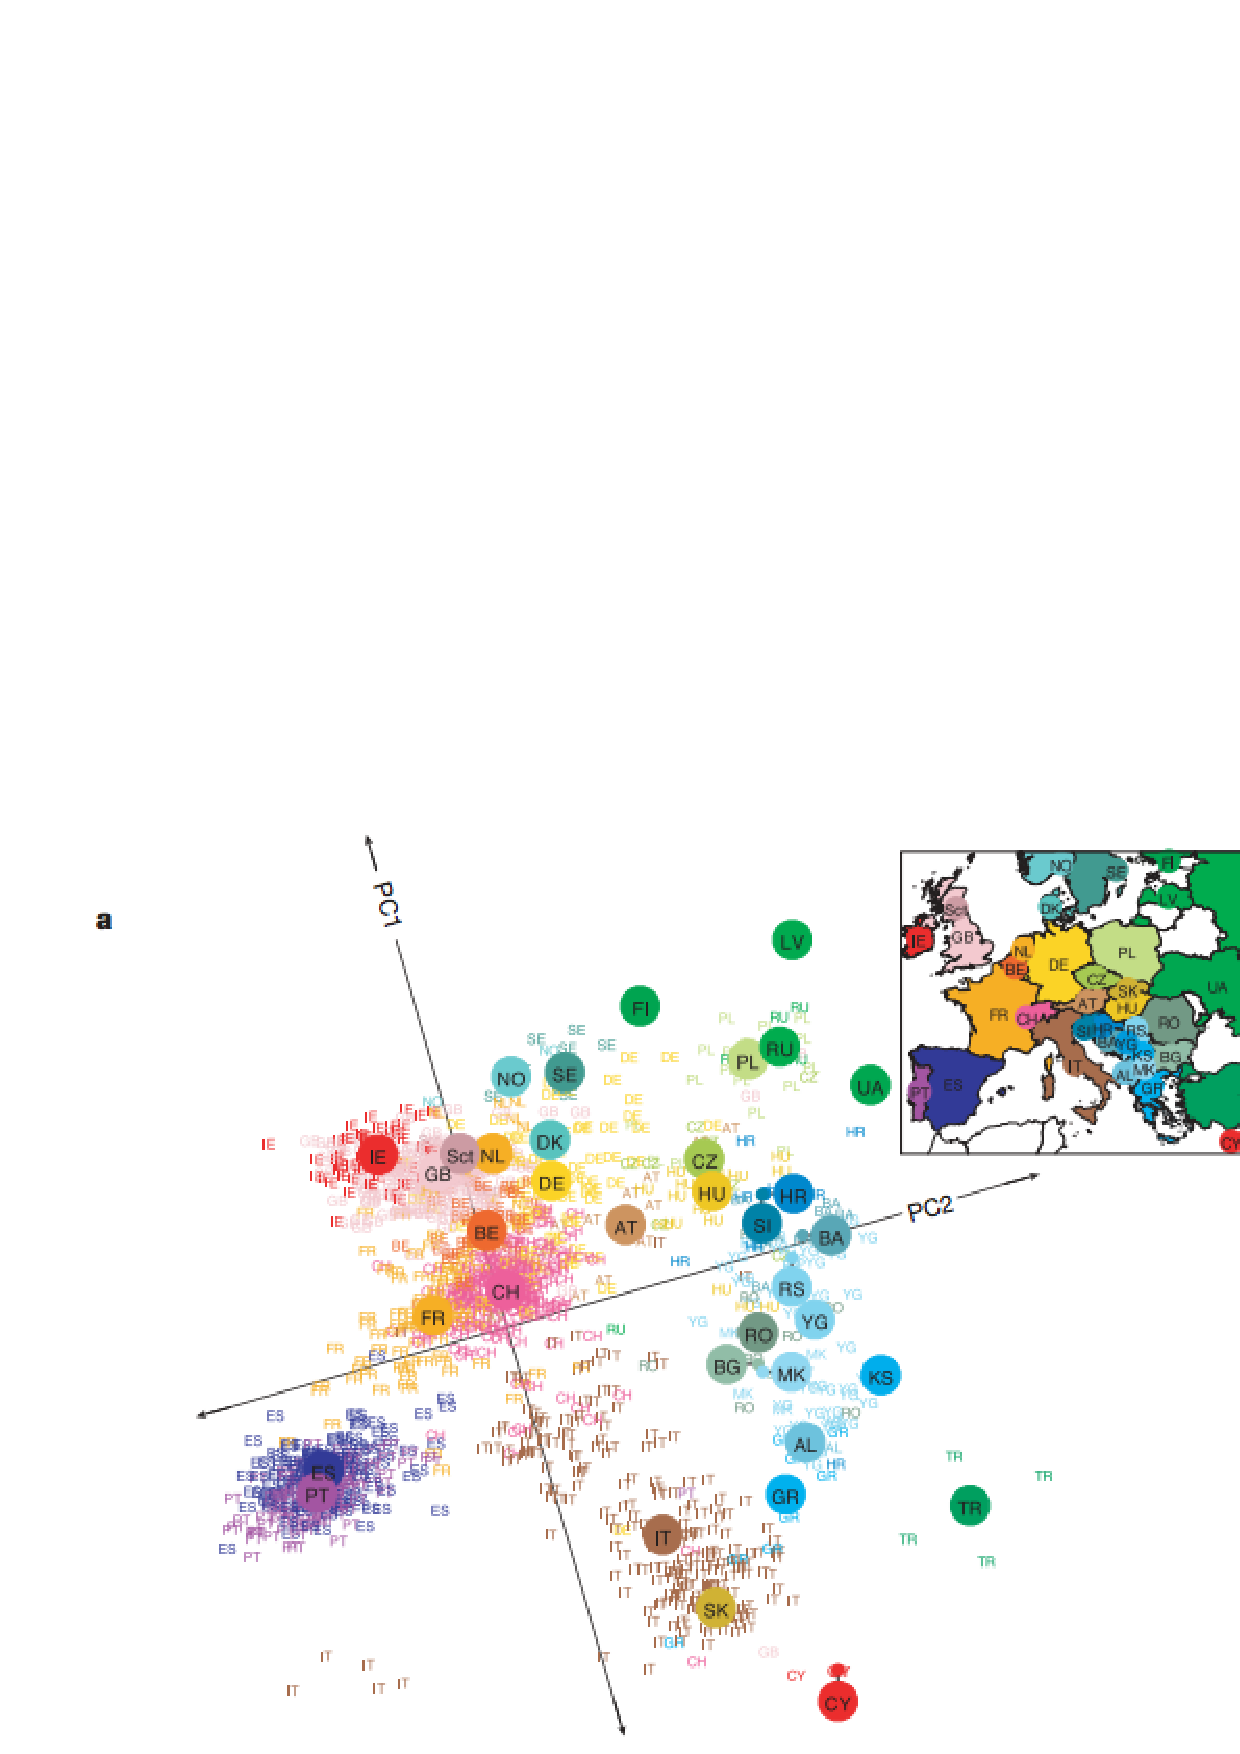
\includegraphics[height = \textheight]{../Figs/Novembre.pdf}
\end{frame}




\begin{frame}[t]
\frametitle{$Q_{ST}/F_{ST}$ in continuously sampled populations}
	\begin{columns}[T] % align columns
		\begin{column}{.42\textwidth}
			\only<1-3>{\includegraphics[height = 4cm]{../Figs/Tree.pdf}}
		\end{column}%
		\hfill%
		\begin{column}{.56\textwidth}
			\begin{block}{$Q_{ST}$}
				\only<1-2>{$Q_{ST} = \frac{V_B}{V_B+V_W}$\\~\\}
				\only<1-2>{$F_{ST} = \mathbb{E}\left[\frac{V_B}{V_B+V_W}\right]$}
				\only<3-3>{$Q_{ST} = \frac{\left(\vec{U}_1\cdot\vec{Z}\right)^2}{\left(\vec{U}_1\cdot\vec{Z}\right)^2 + \sum_{j=2}^K\left(\vec{U}_j\cdot\vec{Z}\right)^2}$\\~\\}
				\only<3-3>{$F_{ST} = \frac{\lambda_1}{\lambda_1 + \sum_{j=2}^K\lambda_j}$}
			\end{block}
		\end{column}%
	\end{columns}
	\only<1-3>{\begin{block}{The Principal Components View}
		\centering$\mathbf{F} = 
					\only<1-2>{\begin{bmatrix}
								\mathbf{F_1}&	\mathbf{0} \\
								\mathbf{0}&	\mathbf{F_2} \\
							\end{bmatrix}}
					\only<3-3>{\begin{bmatrix}
						\vec{U}_1&	\vec{U}_2& \dots&	\vec{U}_K
					\end{bmatrix}
					\begin{bmatrix}
						\lambda_1&	0&	0\\	
						0&	\ddots&	0\\
						0&	0&	\lambda_K
					\end{bmatrix}
					\begin{bmatrix}
						\vec{U}_1^T\\	\vec{U}_2^T\\ \dots\\	\vec{U}_K^T
					\end{bmatrix}}$
	\end{block}}
\end{frame}

\begin{frame}
\frametitle{\normalsize Positive result if population predicts phenotype better than expected}
\only<1-1>{\includegraphics[width = \textwidth]{../Figs/2PopPCPlotPos.pdf}}
\only<2-2>{\includegraphics[width = \textwidth]{../Figs/2PopPCPlotNeg.pdf}}
\end{frame}


\begin{frame}[t]
\frametitle{$Q_{ST}/F_{ST}$ in continuously sampled populations}
	\begin{columns}[T] % align columns
		\begin{column}{.42\textwidth}
			\only<1-1>{\includegraphics[height = 4cm]{../Figs/Tree.pdf}}
			\only<2-3>{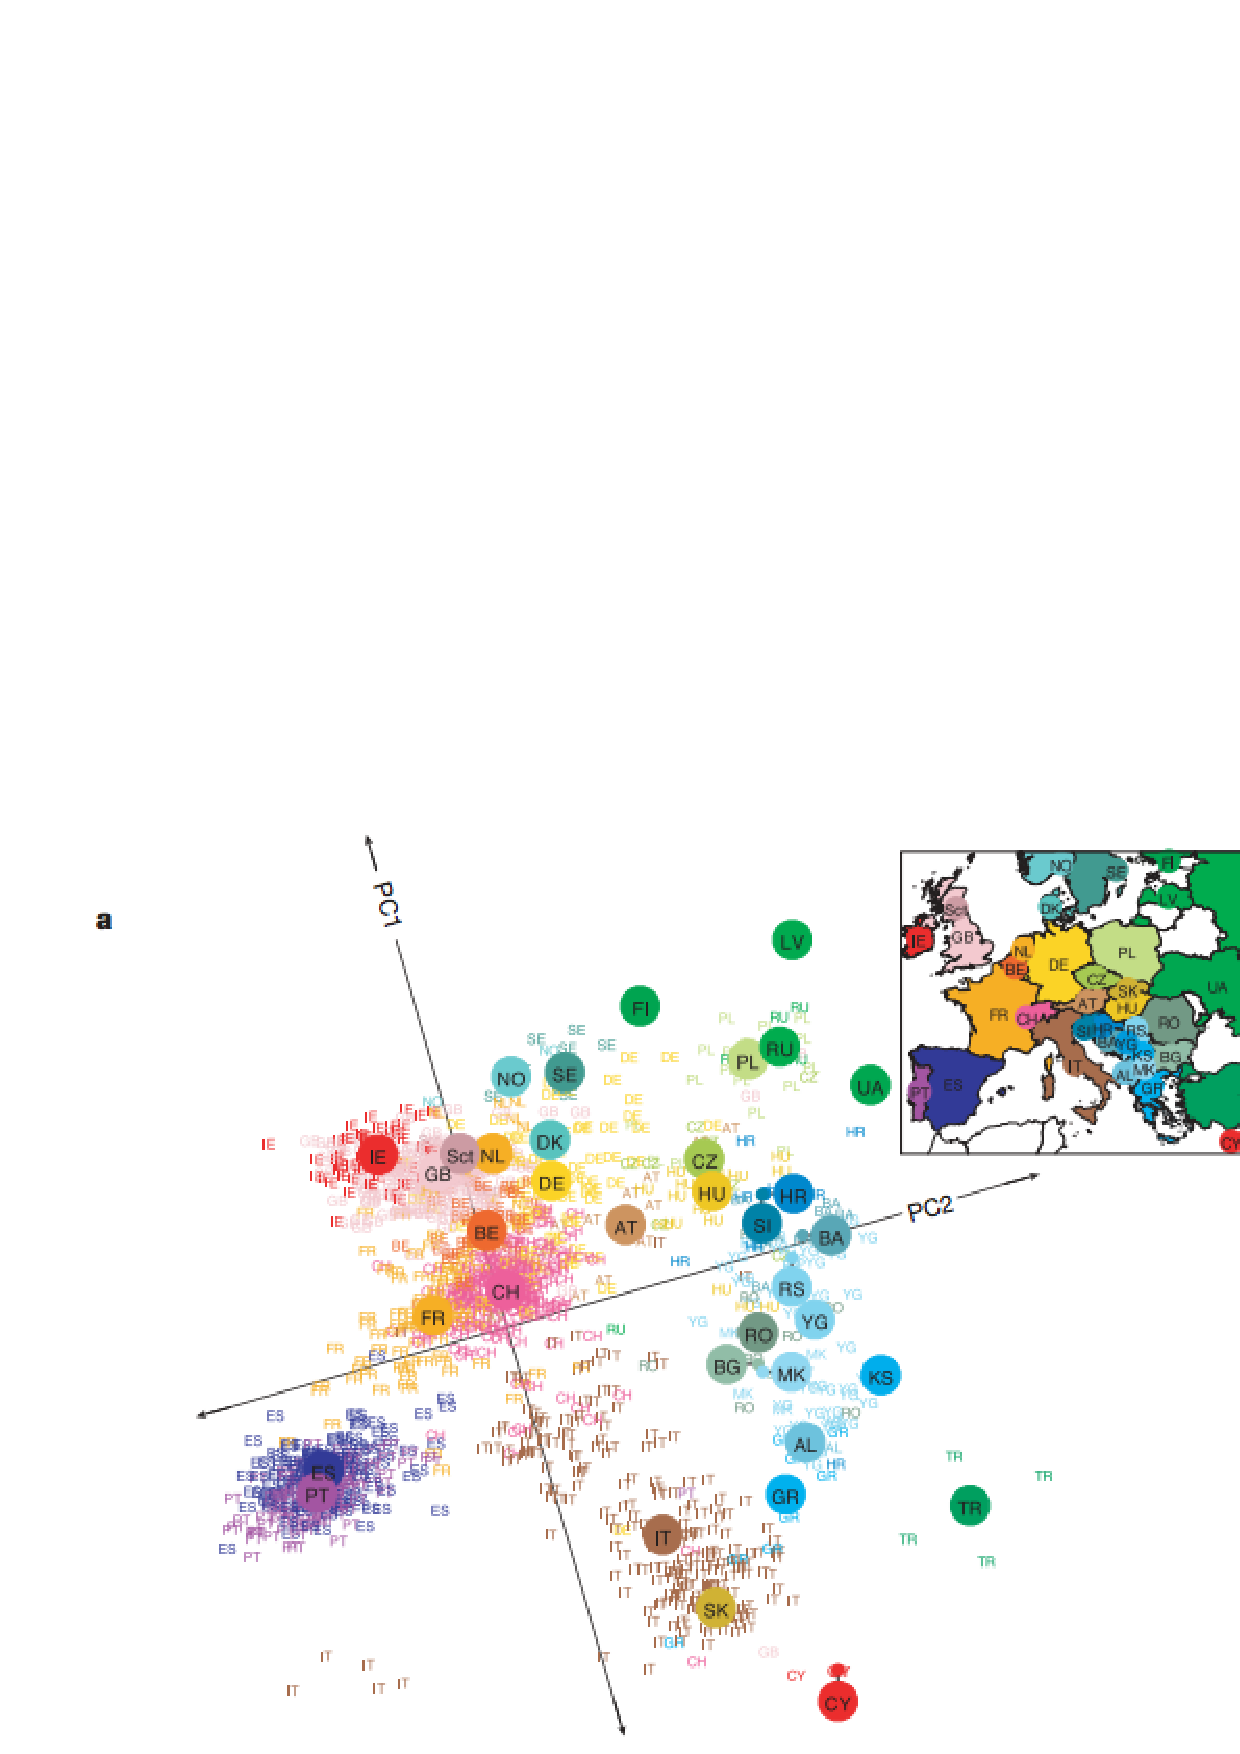
\includegraphics[height = 4cm]{../Figs/Novembre.pdf}}
		\end{column}%
		\hfill%
		\begin{column}{.56\textwidth}
			\begin{block}{$Q_{ST}$}
				\only<1-1>{$Q_{ST} = \frac{\left(\vec{U}_1\cdot\vec{Z}\right)^2}{\left(\vec{U}_i\cdot\vec{Z}\right)^2 + \sum_{j=2}^{K-1}\left(\vec{U}_j\cdot\vec{Z}\right)^2}$\\~\\}
				\only<1-1>{$F_{ST} = \frac{\lambda_1}{\lambda_1 + \sum_{j=2}^{K-1}\lambda_j}$}
				\only<2-2>{$Q_{PC1:2} = \frac{V_{PC1:2}}{V_{PC1:2}+V_{PC3:K-1}}$\\~\\}
				\only<2-2>{$F_{PC1:2} = \mathbb{E}\left[\frac{V_{PC1:2}}{V_{PC1:2}+V_{PC3:K-1}}\right]$}
				\only<3-3>{$Q_{PC1} = \frac{\sum_{i=1}^2\left(\vec{U}_i\cdot\vec{Z}\right)^2}{\sum_{i=1}^2\left(\vec{U}_i\cdot\vec{Z}\right)^2+\sum_{j=3}^{K-1}\left(\vec{U}_j\cdot\vec{Z}\right)^2}$\\~\\}
				\only<3-3>{$F_{PC1} = \frac{\sum_{i=1}^2\lambda_i}{\sum_{i=1}^2\lambda_i + \sum_{j=3}^{K-1}\lambda_j}$}
			\end{block}
		\end{column}%
	\end{columns}
	\only<1-3>{\begin{block}{The Principal Components View}
		\centering$\mathbf{F} = 
					\only<1-3>{\begin{bmatrix}
						\vec{U}_1&	\vec{U}_2& \dots&	\vec{U}_{K-1}
					\end{bmatrix}
					\begin{bmatrix}
						\lambda_1&	0&	0\\	
						0&	\ddots&	0\\
						0&	0&	\lambda_{K-1}
					\end{bmatrix}
					\begin{bmatrix}
						\vec{U}_1^T\\	\vec{U}_2^T\\ \dots\\	\vec{U}_{K-1}^T
					\end{bmatrix}}$
	\end{block}}
\end{frame}


\begin{frame}
\frametitle{Genetic Divergence for Height in Europe}
\only<1-1>{\includegraphics[height = \textheight]{../Figs/QPC12Plot.pdf}}
\only<2-2>{\includegraphics[height = \textheight]{../Figs/QPC12PlotWArrow.pdf}}
\end{frame}

\begin{frame}
\frametitle{Genetic Divergence in Height Along PC1 in Europe}
\only<1-1>{\includegraphics[height = \textheight]{../Figs/HeightPCs12.pdf}}
\only<2-2>{\includegraphics[height = \textheight]{../Figs/HeightPCs1-10.pdf}}
\end{frame}

\begin{frame}
\frametitle{Genetic Divergence in Height Along PC1 in Europe}
\includegraphics[height = \textheight]{../Figs/HeightVPC1.pdf}
\end{frame}

%\begin{frame}
%\frametitle{But None Along Other PCs}
%\includegraphics[height = \textheight]{../Figs/HeightPCs.pdf}
%\end{frame}
%
%\begin{frame}
%\frametitle{But None Along Other PCs}
%\includegraphics[height = \textheight]{../Figs/HeightVPC4.pdf}
%\end{frame}

\begin{frame}
\frametitle{Take Aways}
	\begin{itemize}
		\item Height associated SNPs significantly correlated with PC1/N-S axis in Europe (but we already knew that)
		\pause
		\item $Q_{ST}/F_{ST}$ can be formulated in terms of reduced rank factorizations of the individual-by-individual kinship matrix
			\begin{itemize}
				\item Direct relationship to PCA, \textit{structure}, Sparse Factor Analysis
				\item Engelhardt  and Stephens 2010
			\end{itemize}
	\end{itemize}
\end{frame}


\begin{frame}
	\frametitle{Things I Didn't Mention}
	\begin{itemize}
		\item Can add include multiple correlated traits, but interpretation potentially trickier
		\begin{itemize}
			\item Chenoweth and Blows (2008)
			\item Martin et al (2008)
		\end{itemize}
		\item In species where it's possible to set up breeding designs, continuous sampling is not a barrier
	\end{itemize}
\end{frame}


\begin{frame}
	\frametitle{Acknowledgements}
\end{frame}

%
%\begin{frame}
%\frametitle{The Likelihood Interpretation}
%	\begin{block}{A Simple Generative Model}
%		$$\vec{Z} \sim MVN\left(\vec{0},2V_T\mathbf{F}\right)$$
%		$$\mathbf{F} = \begin{bmatrix}
%						F_{ST}&	0& \dots&	0 \\
%						0&	F_{ST}& \dots&	0 \\
%						\vdots&	\vdots&	\ddots&	\vdots \\
%						0&	0&	\dots&	F_{ST}
%					\end{bmatrix}
%		$$
%	\end{block}
%	\pause\begin{block}{$Q_{ST}/F_{ST}$ as the log-Likelihood of the Data}
%		$$L\left(\vec{Z}\right) = \left(2\pi\right)^{-\frac{M}{2}}\begin{vmatrix}2V_T\mathbf{F}\end{vmatrix}^{-\frac{1}{2}}e^{-\frac{\vec{Z}^T\mathbf{F}^{-1}\vec{Z}}{4V_T}}$$
%		$$-logL\left(\vec{Z}\right) \propto \frac{\vec{Z}^T\mathbf{F}^{-1}\vec{Z}}{2V_T} = \frac{\left(M-1\right)V_B}{\mathbb{E}[V_B]}\sim \chi^2_{M-1}$$
%	\end{block}
%	\pause$Q_{ST}/F_{ST}$ is a measure of the likelihood of the data under a neutral model
%\end{frame}
%
%\begin{frame}
%\frametitle{The Likelihood Interpretation}
%	\begin{block}{A Broader Generative Model}
%		$$\vec{Z} \sim MVN\left(\vec{0},2V_T\mathbf{F}\right)$$
%		$$\mathbf{F} = \begin{bmatrix}
%						f_{11}&	f_{12}& \dots&	f_{1M} \\
%						f_{21}&	f_{22}& \dots&	f_{2M} \\
%						\vdots&	\vdots&	\ddots&	\vdots \\
%						f_{M1}&	f_{M2}&	\dots&	f_{MM}
%					\end{bmatrix}
%		$$
%	\end{block}
%	\pause\begin{block}{$Q_{ST}/F_{ST}$ as the log-Likelihood of the Data}
%		$$L\left(\vec{Z}\right) =\left(2\pi\right)^{-\frac{M}{2}}\begin{vmatrix}2V_T\mathbf{F}\end{vmatrix}^{-\frac{1}{2}}e^{\frac{\vec{Z}^T\mathbf{F}^{-1}\vec{Z}}{2V_T}}$$
%		$$-logL\left(\vec{Z}\right) \propto \frac{\vec{Z}^T\mathbf{F}^{-1}\vec{Z}}{2V_T}$$
%	\end{block}
%\end{frame}
%
%\begin{frame}
%\frametitle{Principal Components Interpetation}
%	\begin{block}{The Principal Components Picture}
%		$$\frac{\vec{Z}^T\mathbf{F}^{-1}\vec{Z}}{2V_T}$$ \\
%		$$\mathbf{F} = \mathbf{U\Lambda U^T}$$ \\
%					$$\mathbf{U\Lambda U^T} = \begin{bmatrix}\vec{u}_1& \vec{u}_2& \dots& \vec{u}_M\end{bmatrix}\begin{bmatrix}
%																		\lambda_1&	0& \dots&	0 \\
%																		0&	\lambda_2& \dots&	0 \\
%																		\vdots&	\vdots&	\ddots&	\vdots \\
%																		0&	0&	\dots&	\lambda_M
%																	\end{bmatrix}\begin{bmatrix}\vec{u}^T_1\\ \vec{u}^T_2\\ \vdots \\ \vec{u}^T_M\end{bmatrix}$$ \\
%		$$\mathbf{F}^{-1} = \mathbf{U\Lambda^{\textmd{-1}} U^T}$$
%	\end{block}
%\end{frame}
%
%
%\begin{frame}
%\frametitle{Principal Components Interpetation}
%	\begin{block}{The Principal Component Picture}
%		$$\mathbf{F}^{-1} = \mathbf{U\Lambda^{\textmd{-1}} U^T}$$ \\
%		\pause\begin{align}
%			\frac{\vec{Z}^T\mathbf{F}^{-1}\vec{Z}}{2V_T} &= \frac{\vec{Z}^T\mathbf{U\Lambda^{\textmd{-1}} U^T}\vec{Z}}{2V_T} \notag \\
%			&= \sum_i \frac{\left(\vec{Z} \cdot \vec{u}_i\right)^2}{2V_T\lambda_i} \notag
%		\end{align}
%		\pause$$\frac{\left(\vec{Z} \cdot \vec{u}_i\right)^2}{2V_T\lambda_i} \sim \chi^2_1$$
%	\end{block}
%\end{frame}
%
%
%
%
%\section{Soft Sweeps}
%
%\begin{frame}
%\frametitle{Soft Sweeps}
%	\begin{figure}
%		\includegraphics[width = \textwidth]{SoftSweepStrongSel.png}
%	\end{figure}
%\end{frame}
%
%\begin{frame}
%\frametitle{Soft Sweeps}
%	\begin{figure}
%		\includegraphics[width = \textwidth]{SoftSweepWeakSel.png}
%	\end{figure}
%\end{frame}
%
%\begin{frame}
%\frametitle{Soft Sweeps}
%	\begin{figure}
%		\includegraphics[width = \textwidth]{SoftSweepStandDel.png}
%	\end{figure}
%\end{frame}
%
%\begin{frame}
%\frametitle{Soft Sweeps}
%	\begin{block}{Reduction in Diversity}
%		Reduction in diversity lessened \\
%		Few high frequency haplotypes \\
%		Slow recovery as new mutations occur and neutral diversity is restored
%	\end{block}
%	\begin{figure}
%		\includegraphics[width = \textwidth]{SoftSweepCartoon}
%	\end{figure}
%\end{frame}
%
%\begin{frame}
%	\frametitle{Soft Sweeps - Effect on Neutral Diversity}
%	\begin{itemize}
%		\item Consider two loci, one selected (B), the other neutral (N), located $l$ bases apart on a chromosome
%		\pause
%		\item A soft sweep has just finished at the B locus. If we choose two alleles at the neutral locus, what is the probability that the sweep forces them to coalesce?
%		\pause
%	\end{itemize}
%	$$Pr(\text{no rec off sweep in N}) \pause Pr(\text{B coalesces before mutating}) $$
%\end{frame}
%
%\begin{frame}
%	\frametitle{Soft Sweeps - Effect on Neutral Diversity}
%	Recombination at A
%		\begin{itemize}
%			\item If $X(t)$ gives the frequency of the sweeping allele class $t$ generations ago (i.e. $X(0) = 1$), then
%		\end{itemize}
%		$$Pr(\text{no rec at N in gen t}) = e^{-(1-X(t))lr_{BP}}$$
%		\pause
%		\begin{align*}
%			Pr(\text{no rec at A over course of sweep}) & = \prod_{t=0}^{t_{start}} e^{-(1-X(t))lr_{BP}} \\
%			& = e^{-\frac{1}{2}T_{fix}lr_{BP}}
%		\end{align*}	
%\end{frame}
%	\frametitle{Soft Sweeps - Effect on Netural Diversity}
%\begin{frame}
%	\frametitle{Soft Sweeps - Effect on Neutral Diversity}
%	Mutation and Coalescence at B
%	\begin{itemize}
%		\item The rates of coalescence and mutation at B are given by
%		\begin{align*}
%			\frac{1}{2NX(t)} \hspace{10mm} \text{and} \hspace{10mm} \frac{2\mu_B}{X(t)}
%		\end{align*}
%		\pause
%		\item The probability of coalescence happening before either lineage mutates is
%		\begin{align*}
%			\frac{\frac{1}{2NX(t)}}{\frac{1}{2NX(t)} + \frac{2\mu_B}{X(t)}} = \frac{1}{1+\theta_B}
%		\end{align*}
%	\end{itemize}
%\end{frame}
%
%\begin{frame}
%	\frametitle{Soft Sweeps - Effect on Neutral Diversity}
%		\begin{itemize}
%			\item The probability that the sweep forces coalescence at B is thus
%			$$\frac{1}{1 + \theta_B}e^{-\frac{1}{2}T_{fix}lr_{BP}}$$
%		\end{itemize}
%\end{frame}
%
%\begin{frame}
%	\frametitle{Soft Sweeps - Effect on Neutral Diversity}
%		\begin{figure}
%			\centering
%			\includegraphics[width = \textwidth, height = 0.87\textheight, keepaspectratio = TRUE]{DiversityReduction}		
%		\end{figure}
%\end{frame}
%
%\begin{frame}
%	\frametitle{Soft Sweeps - Effect on Neutral Diversity}
%		The Recurrent Model
%		\begin{itemize}
%			\item Imagine that sweeps happen homogeneously at each base pair at a rate $\nu_{BP}$
%			\pause
%			\item For a single locus, the per generation rate of coalescence due to sweeps is given by
%			\begin{align*}
%				\nu_{BP}\frac{1}{1 + \theta_B}\int_0^\infty e^{-\frac{1}{2}T_{fix}lr_{BP}}\mathrm{d}l =\frac{2\nu_{BP}}{\left(1+\theta_B\right)r_{BP}T_{fix}}
%			\end{align*}
%		\end{itemize}
%\end{frame}
%
%\begin{frame}
%	\frametitle{Soft Sweeps - Effect on Neutral Diversity}
%	\begin{itemize}
%		\item The expectation of pairwise diversity is given by the mutation rate divided by the coalescence rate. Under neutrality, this is
%		$$\mathbb{E}\left[\pi \right] = \frac{2\mu_N}{\frac{1}{2N}} = \theta_N$$
%		\item Under the recurrent soft sweeps model, this quantity changes to
%		$$\mathbb{E}\left[\pi \right] = \frac{2\mu_N}{\frac{1}{2N} + \frac{2\nu_{BP}}{\left(1+\theta_B\right)r_{BP}T_{fix}}} = \frac{r_{BP}\theta_N}{r_{BP} + \frac{4N\nu_{BP}}{\left(1+\theta_B\right)T_{fix}}}$$
%	\end{itemize}
%\end{frame}
%
%\begin{frame}
%	\frametitle{Other Avenues}
%				\includegraphics[width = \textwidth]{SoftSweepFromNeutral.png}
%
%\end{frame}
%
%
\end{document} 